%%%%%%%%%%%%%%%%%%%%%%%%%%%%%%%%%%%%%%%%%%%%%%%%%%%%%%%%%%%%%%%%%%%%%%%%%%%%%%%%
%2345678901234567890123456789012345678901234567890123456789012345678901234567890
%        1         2         3         4         5         6         7         8

\documentclass[letterpaper, 10 pt, conference]{ieeeconf}  % Comment this line out if you need a4paper

%\documentclass[a4paper, 10pt, conference]{ieeeconf}      % Use this line for a4 paper

\IEEEoverridecommandlockouts                              % This command is only needed if 
                                                          % you want to use the \thanks command

\overrideIEEEmargins                                      % Needed to meet printer requirements.

% See the \addtolength command later in the file to balance the column lengths
% on the last page of the document

% The following packages can be found on http:\\www.ctan.org
%\usepackage{graphics} % for pdf, bitmapped graphics files
%\usepackage{epsfig} % for postscript graphics files
%\usepackage{mathptmx} % assumes new font selection scheme installed
%\usepackage{times} % assumes new font selection scheme installed
%\usepackage{amsmath} % assumes amsmath package installed
%\usepackage{amssymb}  % assumes amsmath package installed
\usepackage{graphicx}
\usepackage[export]{adjustbox}
\graphicspath{ {images/} }


\title{\LARGE \bf
Duckiebot with Blind Navigation
}


\author{YuHsin Wu$^{1}$ and Michael Su$^{2}$% <-this % stops a space
\thanks{*This work was supported by the Robotics Master Program in National Chiao Tung University, Taiwan}% <-this % stops a space
\thanks{$^{1}$YuHsin Wu is with National Chiao Tung University, Taiwan.
        {\tt\small whish713.eed04@g2.nctu.edu.tw}}%
\thanks{$^{2}$Michael Su,
        {\tt\small b.d.researcher@ieee.org}}%
}


\begin{document}



\maketitle
\thispagestyle{empty}
\pagestyle{empty}


\section{INTRODUCTION \& MOTIVATION}

Our goal is to apply duckiebot on blind navigation. The original duckiebot runs according to the yellow and white lines on the road and it can run well in the fixed map. Now we hope that our duckiebot can run on the real world, so that our duckiebot can lead blind people to the destination safely. In our duckiebot, we will equip it with a range sensor Asus Xtion, and replace the original line detector and lane filter with a depth line detector and corresponding lane filter to enable our duckiebot to find where the road is. We hope that the blind people's action won't be limited anymore.

\section{SYSTEM ARCHITECTURE \& EQUIPMENTS}

(team part)

\subsection{SYSTEM ARCHITECTURE}
\begin{figure}[h] % h means put this image here
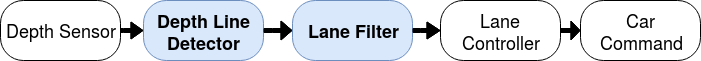
\includegraphics[width=1.0\columnwidth]{system_flowchart.png}
\centering
\caption{system flowchart}
\end{figure}

Generally, we hope that we can keep the original architecture in duckietown lanefollowing. Different from the original version, our depth Line Detector will replace the original line detector and groud projection. The input of Depth Line Detector is pointcloud instead of rgb image. The new detector will detect two walls on both side of road, these two walls are trasformed into line segments which represent the derection of road and is very similar to the line segments in original lanefollowing. 

In original lane filter, the lane width is fixed. To apply depth line detector on the real world, we hope our car is able to run on the road of different width. To achieve this goal, we revise the lane filter to a dynamic-lane-width lane filter. Except the depth line detector and the dynamic-lane-width lane filter, our architecture is the same as the original duckietown.


\subsection{EQUIPMENTS} 

You should list the hardware which is necessary in your project. Your project will only become For example, duckiebot with a gripper Fig.~\ref{figure:duckiebot_gripper}.
\begin{figure}[h] % h means put this image here
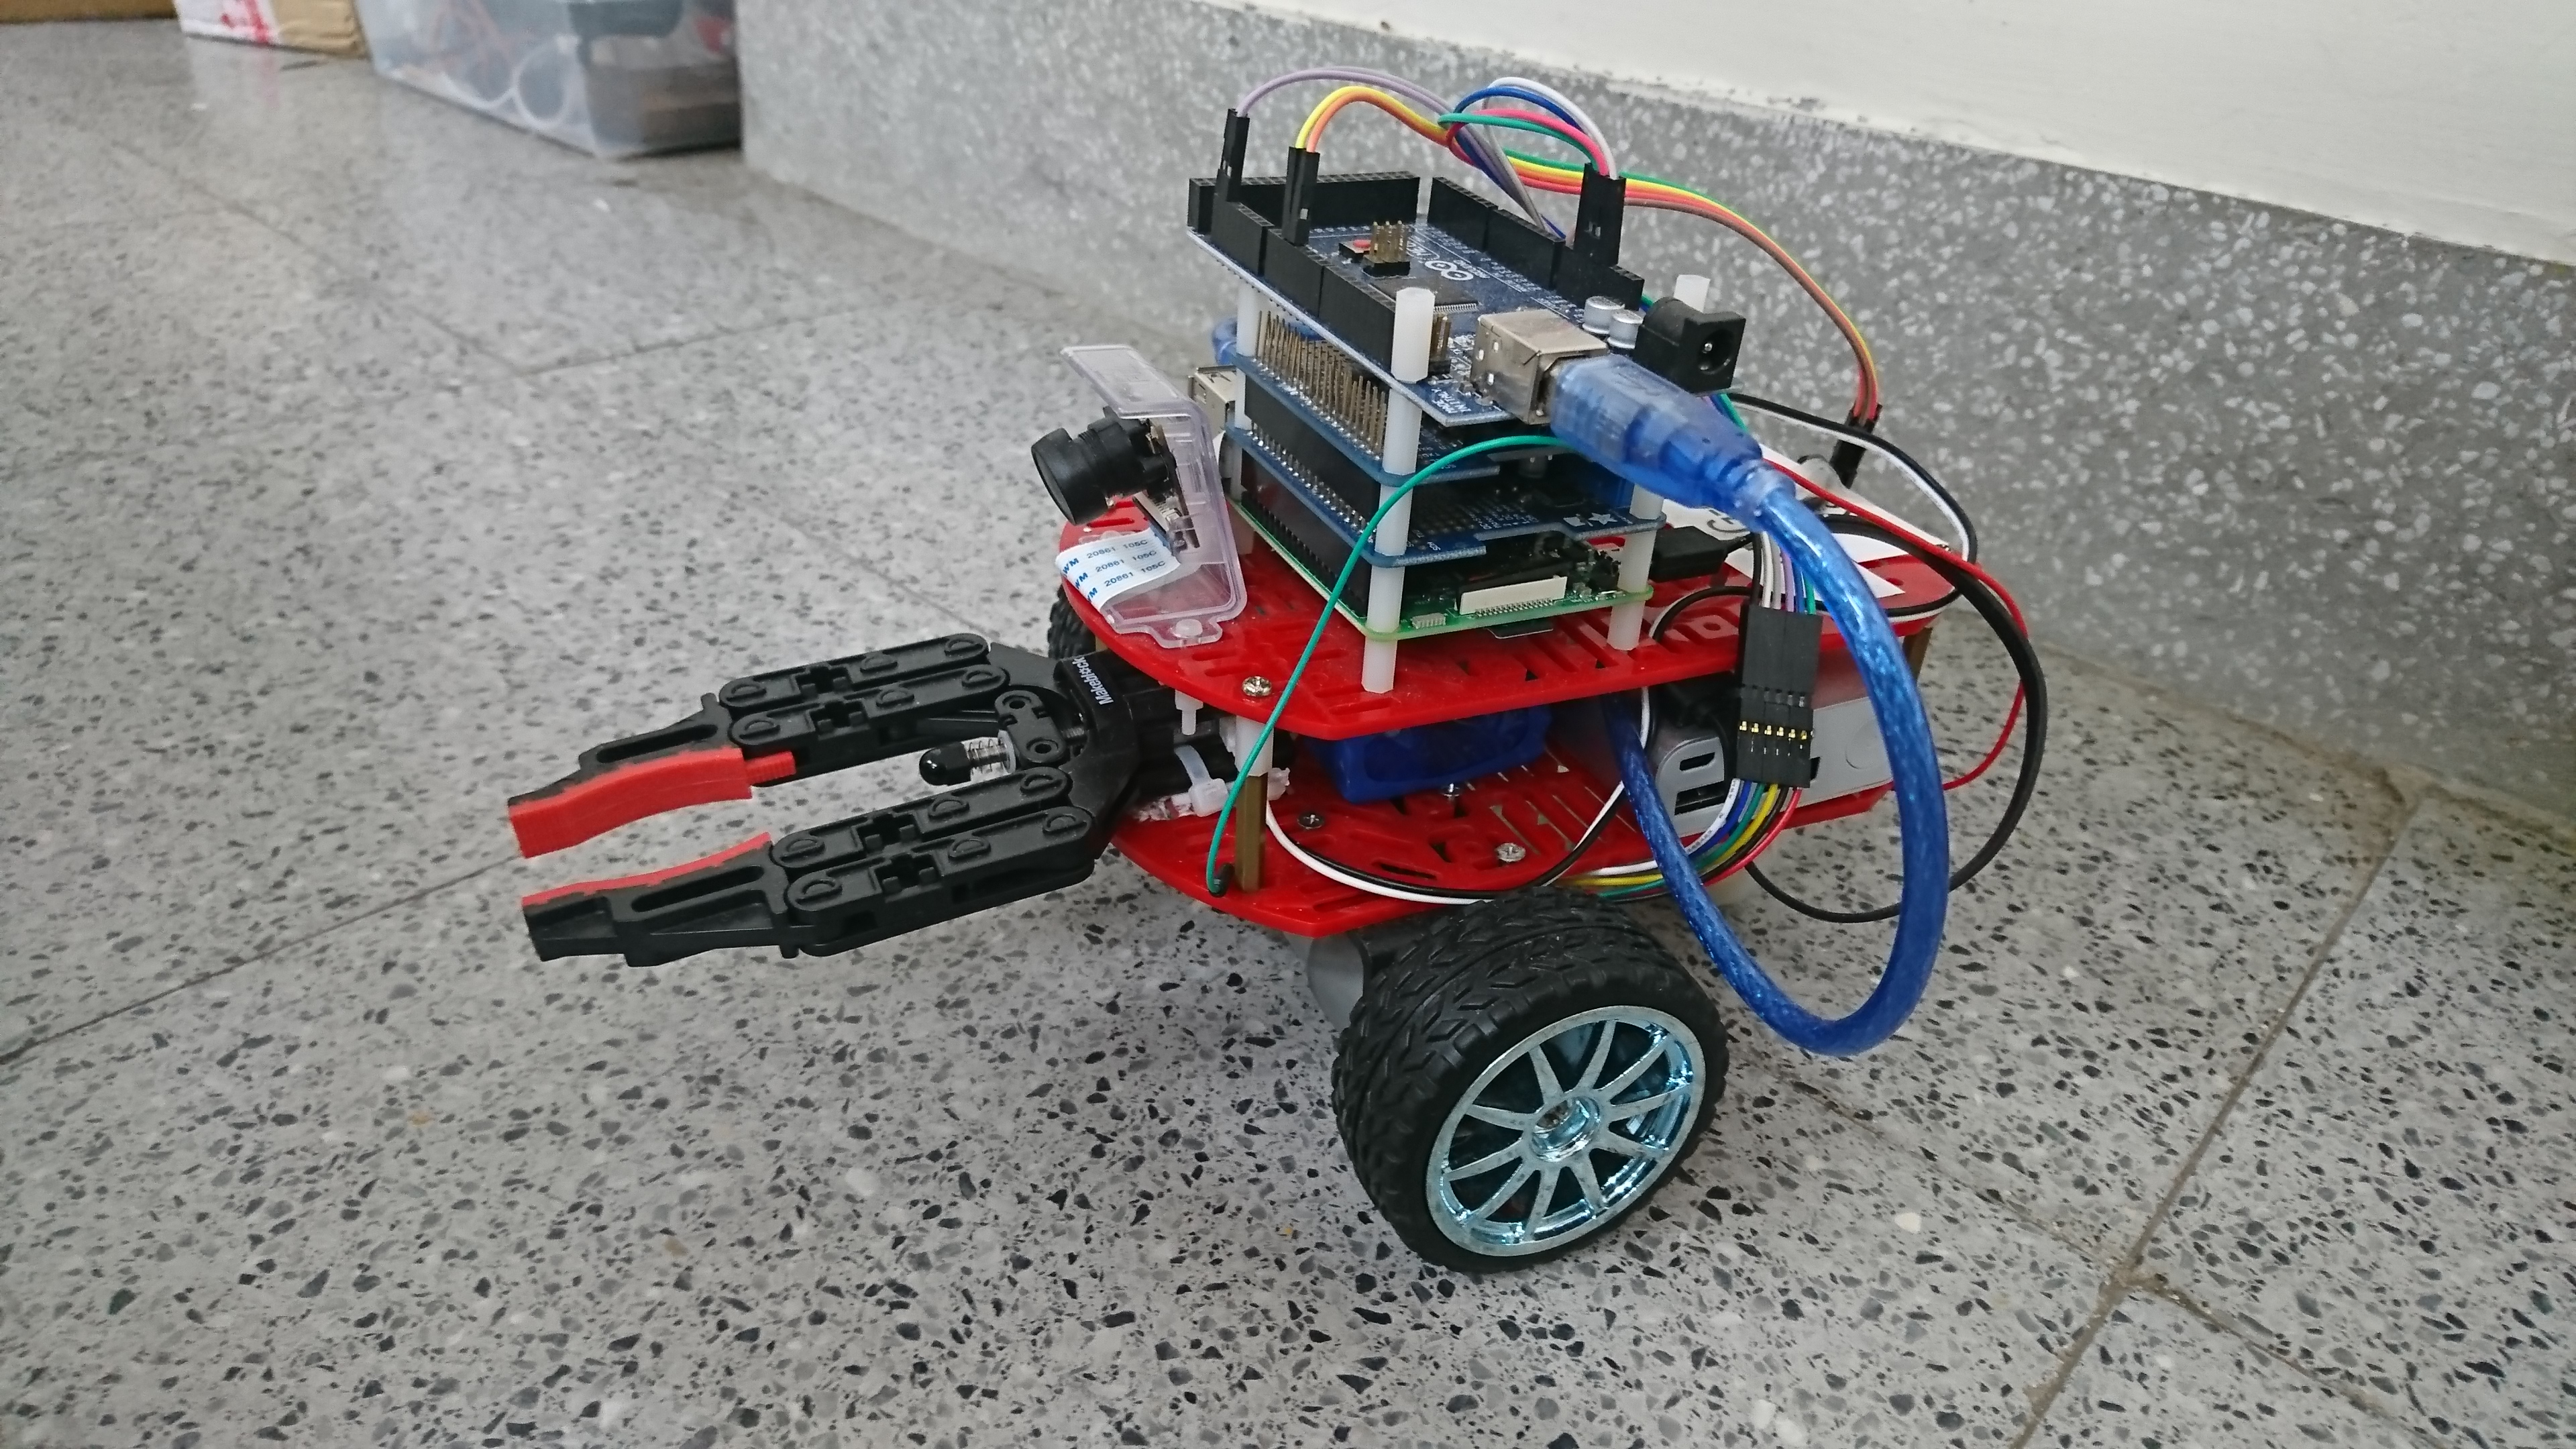
\includegraphics[width=0.8\columnwidth]{duckiebot_gripper}
\centering
\caption{Duckiebot with gripper}
 \label{figure:duckiebot_gripper}
\end{figure}

\begin{figure}[t] % t means put this image at the top 
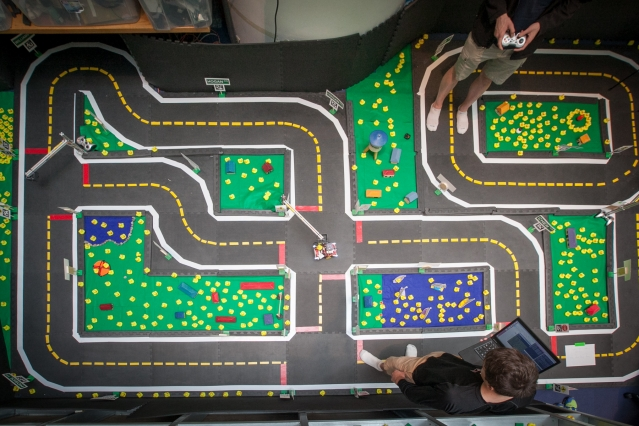
\includegraphics[width=0.8\columnwidth]{duck}
\centering
\caption{Teaser figure: this figure is the most important one in the paper. It gives your readers the first impression of this work. The teaser generally includes the overview of the proposed approach and the key contributions. It appears at the upper right of the first page.}
\end{figure}

\section{SPECIFIC AIMS}

Specific aims need to be concrete enough, so that it is clear what will be the expected outcomes of this work. You also need a reasonable scope that you could finish in this semester.

\begin{itemize}
\item Specific Aim 1.

Dukiebot can go through a map which has fixed lane width.
\item Specific Aim 2.

Dukiebot can go through a map which has dynamic lane width.
\end{itemize}

\section{APPROACH}


\begin{figure}[h] % h means put this image here
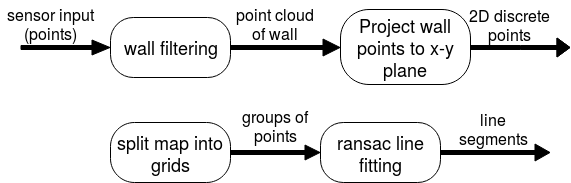
\includegraphics[width=1.0\columnwidth]{approach1.png}
\centering
\caption{approach flowchart}
\end{figure}
1.Wall filtering : Compute the normal of every point, keep points whose normal is horizontal(these points may be the wall part), filter out points whose normal is vertical(these points may be floor or something else).

2.Project wall points : We now have 3D points of wall, but with these points, we can't determine which way to go. So we need to project the wall to x-y plane, then form 2D discrete points. these points imply the trend of wall.  

3.RANSAC line fitting : Model the 2D points into a best line.
\begin{figure}[h] % h means put this image here
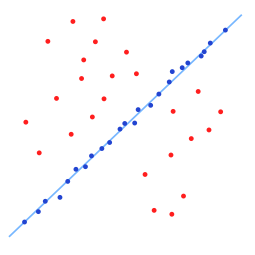
\includegraphics[width=0.5\columnwidth]{RANSAC.png}
\centering
\caption{Fitted line with RANSAC; outliers have no influence on the result.}
\end{figure}

4. Split map : Because the road happens to be curved, we need to split the line, so we can get straight line segments.


\section{SCHEDULE AND TEAM COLLABORATION}

(individual part)

1. Wall filtering	    5days	11/03	11/09

2. Project wall points	5days	11/10	11/16

3. RANSAC line fitting	7days	11/17	11/27

4. Split map	        8days	11/28	12/07

In this section you should write a estimated timeline of your project. This schedule will be very crucial to keep up progress for your project. If you are in a team, you're encouraged to add other team members' on the timeline. It will better show the coordination of your team.
   

\addtolength{\textheight}{-12cm}   % This command serves to balance the column lengths
                                  % on the last page of the document manually. It shortens
                                  % the textheight of the last page by a suitable amount.
                                  % This command does not take effect until the next page
                                  % so it should come on the page before the last. Make
                                  % sure that you do not shorten the textheight too much.

\bibliographystyle{IEEEtran}
\bibliography{egbib}

\end{document}
